\subsection{Resistive Wall Impedance}
\label{sec:res_wall_imp}

The resistive wall impedance is an impedance generated due to the finite conductivity of the material of the beam pipe wall. This can have a number of regimes dependent on whether the skin depth of the material $\delta \left( \omega \right) = \sqrt{\frac{2}{\mu_{0} \sigma \omega}}$ is much smaller than the thickness of the beam pipe wall \cite{Chao:PhysColEff}, comparable to the thickness of the beam pipe wall \cite{Roncarolo:ColImpMeas, Metral:ResWallWideFreq} or much larger than the thickness of the beam pipe wall \cite{Tsutsui:ferrKickLong, Biancacci:MMFiniteInsert}. In this instance, $\sigma$ is the conductivity of wall material. It can also be shown that the shape of the beam pipe cross section also plays a significant role in defining the impedance \cite{Mounet:Axisymmetric, Mounet:Flat}.

Here we shall not attempt a comprehensive summary of the various resistive wall impedance models, but simply give an introduction to the classic thick wall formalism to give a sense of how changing the wall conductivity affects the resistive wall impedance. A considerably more detailed overview of this derivation can be found in \cite{Chao:PhysColEff}. Consider a circular beam pipe of radius $a$ containing a source particle of charge $q_{1}$ moving with velocity $\mathbf{v} = \beta c \mathbf{\hat{z}}$, as shown in Fig.~\ref{fig:res_wall_diagram}. In this case it shall be assumed that $\beta = 1$.

\begin{figure}
\begin{center}
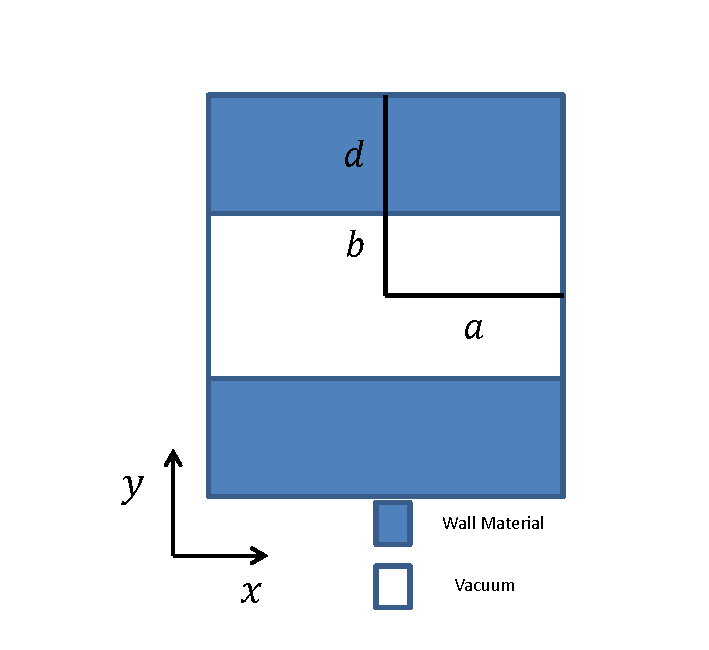
\includegraphics[width=0.8\textwidth]{Wakefields_and_Impedances/figures/reWallGeo.pdf}
\end{center}
\caption{The geometry of the classical thick wall formula.}
\label{fig:res_wall_diagram}
\end{figure}

It can be shown that the beam coupling impedance per unit length $L$ of this structure, assuming $\delta \ll b$, is given by

\begin{align}
\frac{Z_{\parallel}^{0}  \left( \omega \right)}{L} &= \frac{1 - sgn \left( \omega \right) i }{2 \pi a \delta \sigma} \\
\frac{Z_{\perp}^{1}  \left( \omega \right)}{L} &= \frac{c}{\omega}\frac{1 - sgn \left( \omega \right) i }{2 \pi a^{3} \delta \sigma}
\end{align}

where $sgn$ is a function that returns the sign (positive or negative) of the value. The 0 and 1 indicate these modes represent the zeroeth and first azimuthal modes of the source current. It can be easily seen is that the impedance is proportional to $1/ \sqrt{\sigma}$, thereby indicating that materials with a higher conductivity generally give lower beam coupling impedance in the thick wall regime (see Fig.~\ref{fig:resWallImpComp} for a comparison between two sample materials).

\begin{figure}
\subfigure[]{
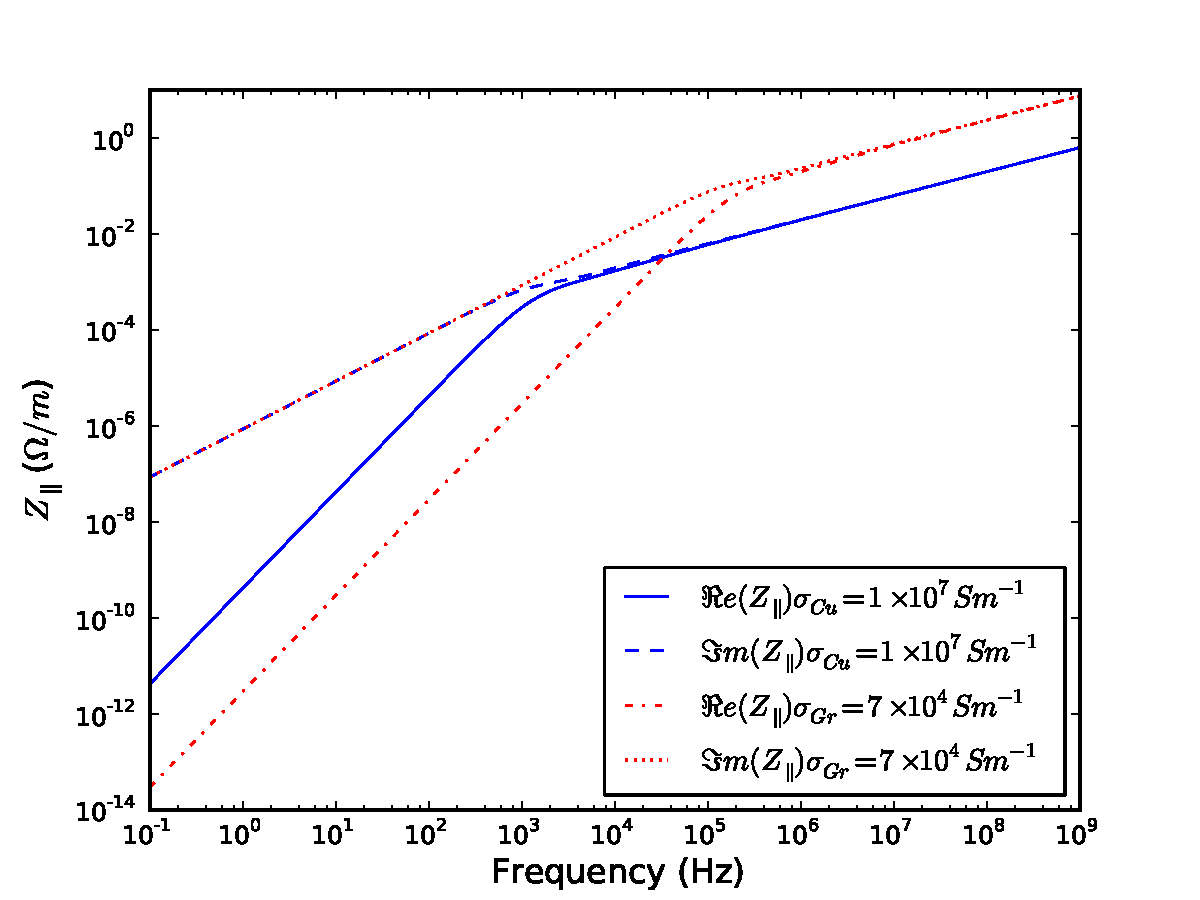
\includegraphics[width=0.5\textwidth]{Wakefields_and_Impedances/figures/resWallTsutsuiLong.pdf}
\label{fig:reswalllong}
}
\subfigure[]{
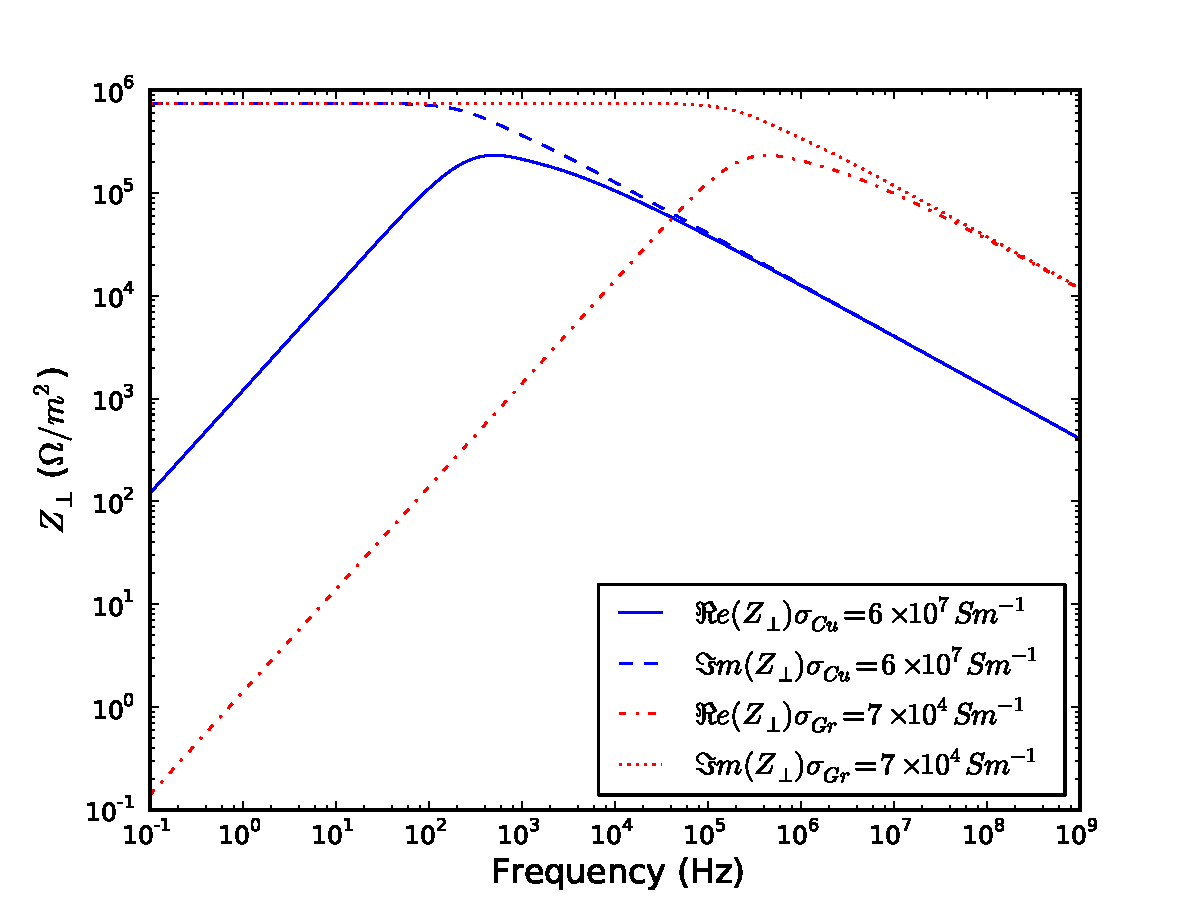
\includegraphics[width=0.5\textwidth]{Wakefields_and_Impedances/figures/resWallTsutsuiTrans.pdf}
\label{fig:reswalltrans}
}

\caption{Examples of the longitudinal \ref{fig:reswalllong} and transverse \ref{fig:reswalltrans} resistive wall impedance of a beam pipe of radius $a = 2cm$ made of both copper ($\sigma = 1 \times 10^{7} S m^{-1}$) and graphite ($\sigma = 7 \times 10^{4} S m^{-1}$).}
\label{fig:resWallImpComp}
\end{figure}

